\documentclass[twoside]{book}

% Packages required by doxygen
\usepackage{fixltx2e}
\usepackage{calc}
\usepackage{doxygen}
\usepackage[export]{adjustbox} % also loads graphicx
\usepackage{graphicx}
\usepackage[utf8]{inputenc}
\usepackage{makeidx}
\usepackage{multicol}
\usepackage{multirow}
\PassOptionsToPackage{warn}{textcomp}
\usepackage{textcomp}
\usepackage[nointegrals]{wasysym}
\usepackage[table]{xcolor}

% Font selection
\usepackage[T1]{fontenc}
\usepackage[scaled=.90]{helvet}
\usepackage{courier}
\usepackage{amssymb}
\usepackage{sectsty}
\renewcommand{\familydefault}{\sfdefault}
\allsectionsfont{%
  \fontseries{bc}\selectfont%
  \color{darkgray}%
}
\renewcommand{\DoxyLabelFont}{%
  \fontseries{bc}\selectfont%
  \color{darkgray}%
}
\newcommand{\+}{\discretionary{\mbox{\scriptsize$\hookleftarrow$}}{}{}}

% Page & text layout
\usepackage{geometry}
\geometry{%
  a4paper,%
  top=2.5cm,%
  bottom=2.5cm,%
  left=2.5cm,%
  right=2.5cm%
}
\tolerance=750
\hfuzz=15pt
\hbadness=750
\setlength{\emergencystretch}{15pt}
\setlength{\parindent}{0cm}
\setlength{\parskip}{3ex plus 2ex minus 2ex}
\makeatletter
\renewcommand{\paragraph}{%
  \@startsection{paragraph}{4}{0ex}{-1.0ex}{1.0ex}{%
    \normalfont\normalsize\bfseries\SS@parafont%
  }%
}
\renewcommand{\subparagraph}{%
  \@startsection{subparagraph}{5}{0ex}{-1.0ex}{1.0ex}{%
    \normalfont\normalsize\bfseries\SS@subparafont%
  }%
}
\makeatother

% Headers & footers
\usepackage{fancyhdr}
\pagestyle{fancyplain}
\fancyhead[LE]{\fancyplain{}{\bfseries\thepage}}
\fancyhead[CE]{\fancyplain{}{}}
\fancyhead[RE]{\fancyplain{}{\bfseries\leftmark}}
\fancyhead[LO]{\fancyplain{}{\bfseries\rightmark}}
\fancyhead[CO]{\fancyplain{}{}}
\fancyhead[RO]{\fancyplain{}{\bfseries\thepage}}
\fancyfoot[LE]{\fancyplain{}{}}
\fancyfoot[CE]{\fancyplain{}{}}
\fancyfoot[RE]{\fancyplain{}{\bfseries\scriptsize Generated by Doxygen }}
\fancyfoot[LO]{\fancyplain{}{\bfseries\scriptsize Generated by Doxygen }}
\fancyfoot[CO]{\fancyplain{}{}}
\fancyfoot[RO]{\fancyplain{}{}}
\renewcommand{\footrulewidth}{0.4pt}
\renewcommand{\chaptermark}[1]{%
  \markboth{#1}{}%
}
\renewcommand{\sectionmark}[1]{%
  \markright{\thesection\ #1}%
}

% Indices & bibliography
\usepackage{natbib}
\usepackage[titles]{tocloft}
\setcounter{tocdepth}{3}
\setcounter{secnumdepth}{5}
\makeindex

% Hyperlinks (required, but should be loaded last)
\usepackage{ifpdf}
\ifpdf
  \usepackage[pdftex,pagebackref=true]{hyperref}
\else
  \usepackage[ps2pdf,pagebackref=true]{hyperref}
\fi
\hypersetup{%
  colorlinks=true,%
  linkcolor=blue,%
  citecolor=blue,%
  unicode%
}

% Custom commands
\newcommand{\clearemptydoublepage}{%
  \newpage{\pagestyle{empty}\cleardoublepage}%
}

\usepackage{caption}
\captionsetup{labelsep=space,justification=centering,font={bf},singlelinecheck=off,skip=4pt,position=top}

%===== C O N T E N T S =====

\begin{document}

% Titlepage & ToC
\hypersetup{pageanchor=false,
             bookmarksnumbered=true,
             pdfencoding=unicode
            }
\pagenumbering{alph}
\begin{titlepage}
\vspace*{7cm}
\begin{center}%
{\Large Project 7 }\\
\vspace*{1cm}
{\large Generated by Doxygen 1.8.12}\\
\end{center}
\end{titlepage}
\clearemptydoublepage
\pagenumbering{roman}
\tableofcontents
\clearemptydoublepage
\pagenumbering{arabic}
\hypersetup{pageanchor=true}

%--- Begin generated contents ---
\chapter{Hierarchical Index}
\section{Class Hierarchy}
This inheritance list is sorted roughly, but not completely, alphabetically\+:\begin{DoxyCompactList}
\item \contentsline{section}{Binary\+Node$<$ Item\+Type $>$}{\pageref{class_binary_node}}{}
\item \contentsline{section}{Binary\+Node\+Tree$<$ Item\+Type $>$}{\pageref{class_binary_node_tree}}{}
\begin{DoxyCompactList}
\item \contentsline{section}{Binary\+Search\+Tree$<$ Item\+Type $>$}{\pageref{class_binary_search_tree}}{}
\end{DoxyCompactList}
\end{DoxyCompactList}

\chapter{Class Index}
\subsection{Class List}
Here are the classes, structs, unions and interfaces with brief descriptions\+:\begin{DoxyCompactList}
\item\contentsline{section}{\hyperlink{class_linked_list}{Linked\+List$<$ Item\+Type $>$} }{\pageref{class_linked_list}}{}
\item\contentsline{section}{\hyperlink{class_list_interface}{List\+Interface$<$ Item\+Type $>$} }{\pageref{class_list_interface}}{}
\item\contentsline{section}{\hyperlink{class_node}{Node$<$ Item\+Type $>$} }{\pageref{class_node}}{}
\item\contentsline{section}{\hyperlink{class_precond_violated_except}{Precond\+Violated\+Except} }{\pageref{class_precond_violated_except}}{}
\end{DoxyCompactList}

\chapter{File Index}
\section{File List}
Here is a list of all documented files with brief descriptions\+:\begin{DoxyCompactList}
\item\contentsline{section}{\hyperlink{_binary_node_8cpp}{Binary\+Node.\+cpp} \\*Implementation file for the Binary Node class }{\pageref{_binary_node_8cpp}}{}
\item\contentsline{section}{\hyperlink{_binary_node_8h}{Binary\+Node.\+h} \\*Header file for the Binary Node class }{\pageref{_binary_node_8h}}{}
\item\contentsline{section}{\hyperlink{_binary_node_tree_8cpp}{Binary\+Node\+Tree.\+cpp} \\*Implementation file for the Binary Node Tree class }{\pageref{_binary_node_tree_8cpp}}{}
\item\contentsline{section}{\hyperlink{_binary_node_tree_8h}{Binary\+Node\+Tree.\+h} \\*Header file for the Binary Node Tree class }{\pageref{_binary_node_tree_8h}}{}
\item\contentsline{section}{\hyperlink{_binary_search_tree_8cpp}{Binary\+Search\+Tree.\+cpp} \\*Implementation file for the Binary Search Tree class }{\pageref{_binary_search_tree_8cpp}}{}
\item\contentsline{section}{\hyperlink{_binary_search_tree_8h}{Binary\+Search\+Tree.\+h} \\*Header file for the Binary Search Tree class }{\pageref{_binary_search_tree_8h}}{}
\item\contentsline{section}{\hyperlink{_p_a07_8cpp}{P\+A07.\+cpp} \\*Main driver for project 7 }{\pageref{_p_a07_8cpp}}{}
\item\contentsline{section}{\hyperlink{_red_black_tree_8cpp}{Red\+Black\+Tree.\+cpp} \\*Implementation file for the Red Black Tree class }{\pageref{_red_black_tree_8cpp}}{}
\item\contentsline{section}{\hyperlink{_red_black_tree_8h}{Red\+Black\+Tree.\+h} \\*Header file for the Red Black Tree class }{\pageref{_red_black_tree_8h}}{}
\end{DoxyCompactList}

\chapter{Class Documentation}
\hypertarget{class_binary_node}{}\section{Binary\+Node$<$ Item\+Type $>$ Class Template Reference}
\label{class_binary_node}\index{Binary\+Node$<$ Item\+Type $>$@{Binary\+Node$<$ Item\+Type $>$}}
\subsection*{Public Member Functions}
\begin{DoxyCompactItemize}
\item 
void \hyperlink{class_binary_node_ab731c8cf87040e19ecba80f407b4d9b1}{set\+Item} (const Item\+Type \&an\+Item)
\item 
Item\+Type \hyperlink{class_binary_node_a10780d779ff7a9c51473715967a7a439}{get\+Item} () const
\item 
bool \hyperlink{class_binary_node_a837d4805b46040906b8c5a331e73abee}{is\+Leaf} () const
\item 
\hypertarget{class_binary_node_aa6757b8f7b050c4016d15c01bcab805a}{}\label{class_binary_node_aa6757b8f7b050c4016d15c01bcab805a} 
\hyperlink{class_binary_node}{Binary\+Node}$<$ Item\+Type $>$ $\ast$ {\bfseries get\+Parent\+Ptr} () const
\item 
\hypertarget{class_binary_node_acf93048be8864cf90c02dca1106902df}{}\label{class_binary_node_acf93048be8864cf90c02dca1106902df} 
\hyperlink{class_binary_node}{Binary\+Node}$<$ Item\+Type $>$ $\ast$ {\bfseries get\+Left\+Child\+Ptr} () const
\item 
\hypertarget{class_binary_node_ad96f01da47b6786a5f4f384380755c96}{}\label{class_binary_node_ad96f01da47b6786a5f4f384380755c96} 
\hyperlink{class_binary_node}{Binary\+Node}$<$ Item\+Type $>$ $\ast$ {\bfseries get\+Right\+Child\+Ptr} () const
\item 
\hypertarget{class_binary_node_a5df87a46296c99ed99444996ee7bbff6}{}\label{class_binary_node_a5df87a46296c99ed99444996ee7bbff6} 
void {\bfseries set\+Parent\+Ptr} (\hyperlink{class_binary_node}{Binary\+Node}$<$ Item\+Type $>$ $\ast$parent\+Ptr)
\item 
\hypertarget{class_binary_node_aa36a2b61c6b76aeb79465776c80d5c49}{}\label{class_binary_node_aa36a2b61c6b76aeb79465776c80d5c49} 
void {\bfseries set\+Left\+Child\+Ptr} (\hyperlink{class_binary_node}{Binary\+Node}$<$ Item\+Type $>$ $\ast$left\+Ptr)
\item 
\hypertarget{class_binary_node_a2252f471ea06bb2568b6c2af5ece23f6}{}\label{class_binary_node_a2252f471ea06bb2568b6c2af5ece23f6} 
void {\bfseries set\+Right\+Child\+Ptr} (\hyperlink{class_binary_node}{Binary\+Node}$<$ Item\+Type $>$ $\ast$right\+Ptr)
\end{DoxyCompactItemize}
\subsection*{Public Attributes}
\begin{DoxyCompactItemize}
\item 
\hypertarget{class_binary_node_a11390eb78e60c4a61b0c54dcf743063a}{}\label{class_binary_node_a11390eb78e60c4a61b0c54dcf743063a} 
color\+\_\+t {\bfseries color}
\end{DoxyCompactItemize}


\subsection{Member Function Documentation}
\hypertarget{class_binary_node_a10780d779ff7a9c51473715967a7a439}{}\label{class_binary_node_a10780d779ff7a9c51473715967a7a439} 
\index{Binary\+Node@{Binary\+Node}!get\+Item@{get\+Item}}
\index{get\+Item@{get\+Item}!Binary\+Node@{Binary\+Node}}
\subsubsection{\texorpdfstring{get\+Item()}{getItem()}}
{\footnotesize\ttfamily template$<$class Item\+Type $>$ \\
Item\+Type \hyperlink{class_binary_node}{Binary\+Node}$<$ Item\+Type $>$\+::get\+Item (\begin{DoxyParamCaption}{ }\end{DoxyParamCaption}) const}

Returns the item data member \begin{DoxyReturn}{Returns}
The item data member. 
\end{DoxyReturn}
\hypertarget{class_binary_node_a837d4805b46040906b8c5a331e73abee}{}\label{class_binary_node_a837d4805b46040906b8c5a331e73abee} 
\index{Binary\+Node@{Binary\+Node}!is\+Leaf@{is\+Leaf}}
\index{is\+Leaf@{is\+Leaf}!Binary\+Node@{Binary\+Node}}
\subsubsection{\texorpdfstring{is\+Leaf()}{isLeaf()}}
{\footnotesize\ttfamily template$<$class Item\+Type $>$ \\
bool \hyperlink{class_binary_node}{Binary\+Node}$<$ Item\+Type $>$\+::is\+Leaf (\begin{DoxyParamCaption}{ }\end{DoxyParamCaption}) const}

Tells if the node is a leaf \begin{DoxyReturn}{Returns}
Whether or not the node is a leaf of the tree. 
\end{DoxyReturn}
\hypertarget{class_binary_node_ab731c8cf87040e19ecba80f407b4d9b1}{}\label{class_binary_node_ab731c8cf87040e19ecba80f407b4d9b1} 
\index{Binary\+Node@{Binary\+Node}!set\+Item@{set\+Item}}
\index{set\+Item@{set\+Item}!Binary\+Node@{Binary\+Node}}
\subsubsection{\texorpdfstring{set\+Item()}{setItem()}}
{\footnotesize\ttfamily template$<$class Item\+Type $>$ \\
void \hyperlink{class_binary_node}{Binary\+Node}$<$ Item\+Type $>$\+::set\+Item (\begin{DoxyParamCaption}\item[{const Item\+Type \&}]{an\+Item }\end{DoxyParamCaption})}

Sets the item data member 

The documentation for this class was generated from the following files\+:\begin{DoxyCompactItemize}
\item 
\hyperlink{_binary_node_8h}{Binary\+Node.\+h}\item 
\hyperlink{_binary_node_8cpp}{Binary\+Node.\+cpp}\end{DoxyCompactItemize}

\hypertarget{class_binary_node_tree}{}\section{Binary\+Node\+Tree$<$ Item\+Type $>$ Class Template Reference}
\label{class_binary_node_tree}\index{Binary\+Node\+Tree$<$ Item\+Type $>$@{Binary\+Node\+Tree$<$ Item\+Type $>$}}
Inheritance diagram for Binary\+Node\+Tree$<$ Item\+Type $>$\+:\begin{figure}[H]
\begin{center}
\leavevmode
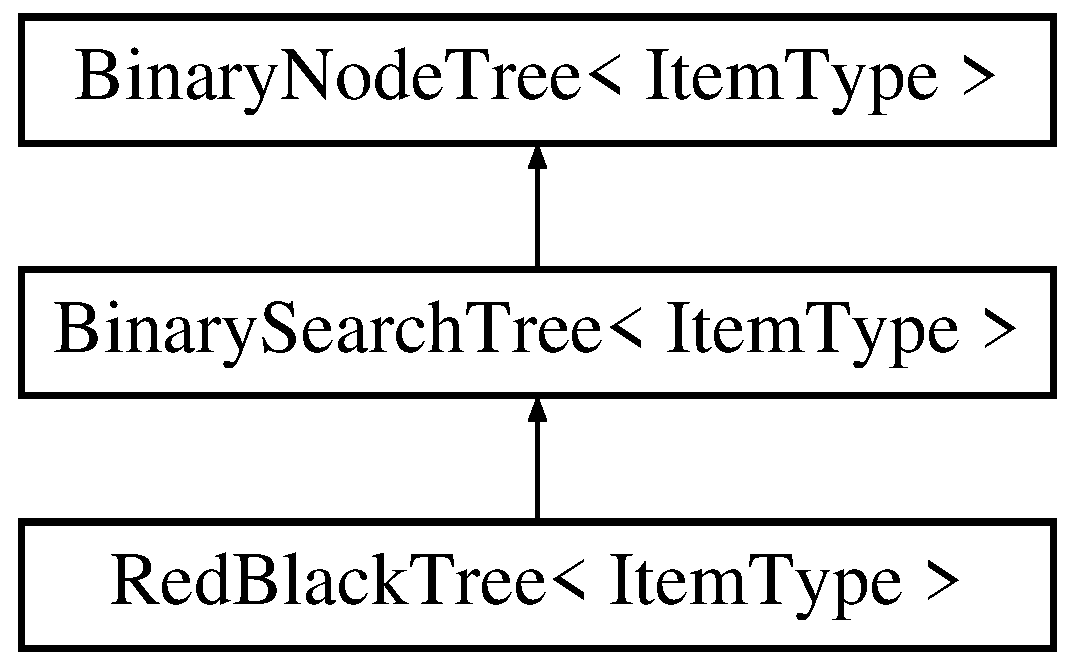
\includegraphics[height=3.000000cm]{class_binary_node_tree}
\end{center}
\end{figure}
\subsection*{Public Member Functions}
\begin{DoxyCompactItemize}
\item 
\hypertarget{class_binary_node_tree_ae3b5ffa874ac164a50dd9cd1eb43ca03}{}\label{class_binary_node_tree_ae3b5ffa874ac164a50dd9cd1eb43ca03} 
bool {\bfseries is\+Empty} () const
\item 
\hypertarget{class_binary_node_tree_a19f562021609b30955f808759f53ca8f}{}\label{class_binary_node_tree_a19f562021609b30955f808759f53ca8f} 
int {\bfseries get\+Height} () const
\item 
\hypertarget{class_binary_node_tree_a2be8730b32f32250c5feff576378d34a}{}\label{class_binary_node_tree_a2be8730b32f32250c5feff576378d34a} 
int {\bfseries get\+Number\+Of\+Nodes} () const
\item 
\hypertarget{class_binary_node_tree_ae8556653f8a673c5fe7a2404948e408f}{}\label{class_binary_node_tree_ae8556653f8a673c5fe7a2404948e408f} 
Item\+Type {\bfseries get\+Root\+Data} () const
\item 
\hypertarget{class_binary_node_tree_a2c839fd1f9eff387ea134792ecb8c34d}{}\label{class_binary_node_tree_a2c839fd1f9eff387ea134792ecb8c34d} 
void {\bfseries set\+Root\+Data} (const Item\+Type \&new\+Data)
\item 
\hypertarget{class_binary_node_tree_a0f98a30d162875a4d5ffedd40b658240}{}\label{class_binary_node_tree_a0f98a30d162875a4d5ffedd40b658240} 
bool {\bfseries add} (const Item\+Type \&new\+Data)
\item 
\hypertarget{class_binary_node_tree_a5c3383e6cde4f794028e2264cd8e9d3f}{}\label{class_binary_node_tree_a5c3383e6cde4f794028e2264cd8e9d3f} 
bool {\bfseries remove} (const Item\+Type \&data)
\item 
\hypertarget{class_binary_node_tree_a6ec544a0b10d9323b8008660825b98b7}{}\label{class_binary_node_tree_a6ec544a0b10d9323b8008660825b98b7} 
void {\bfseries clear} ()
\item 
\hypertarget{class_binary_node_tree_a0231a6e71abac98bb4cca6a0df444c46}{}\label{class_binary_node_tree_a0231a6e71abac98bb4cca6a0df444c46} 
Item\+Type {\bfseries get\+Entry} (const Item\+Type \&an\+Entry) const
\item 
\hypertarget{class_binary_node_tree_a73c482860c5dc6c0b8cec6af720f6cc9}{}\label{class_binary_node_tree_a73c482860c5dc6c0b8cec6af720f6cc9} 
bool {\bfseries contains} (const Item\+Type \&an\+Entry) const
\item 
\hypertarget{class_binary_node_tree_aadc0ac498739400c97d86440c6b5a721}{}\label{class_binary_node_tree_aadc0ac498739400c97d86440c6b5a721} 
void {\bfseries preorder\+Traverse} (void visit(Item\+Type \&)) const
\item 
\hypertarget{class_binary_node_tree_a910b0d440f78a109d0f158b0bd4c36f4}{}\label{class_binary_node_tree_a910b0d440f78a109d0f158b0bd4c36f4} 
void {\bfseries inorder\+Traverse} (void visit(Item\+Type \&)) const
\item 
\hypertarget{class_binary_node_tree_aee55076ce323c43e18776a724943a75f}{}\label{class_binary_node_tree_aee55076ce323c43e18776a724943a75f} 
void {\bfseries postorder\+Traverse} (void visit(Item\+Type \&)) const
\item 
\hypertarget{class_binary_node_tree_a79c6b41ab96eee8649ed29e04b9b699a}{}\label{class_binary_node_tree_a79c6b41ab96eee8649ed29e04b9b699a} 
\hyperlink{class_binary_node_tree}{Binary\+Node\+Tree} \& {\bfseries operator=} (const \hyperlink{class_binary_node_tree}{Binary\+Node\+Tree} \&rhs)
\end{DoxyCompactItemize}
\subsection*{Protected Member Functions}
\begin{DoxyCompactItemize}
\item 
\hypertarget{class_binary_node_tree_ab4fb3e839f07f821d7c1e038758cc111}{}\label{class_binary_node_tree_ab4fb3e839f07f821d7c1e038758cc111} 
int {\bfseries get\+Height\+Helper} (\hyperlink{class_binary_node}{Binary\+Node}$<$ Item\+Type $>$ $\ast$sub\+Tree\+Ptr) const
\item 
\hypertarget{class_binary_node_tree_a924b9aaeb31752e5fcfc2177726d2c58}{}\label{class_binary_node_tree_a924b9aaeb31752e5fcfc2177726d2c58} 
int {\bfseries get\+Number\+Of\+Nodes\+Helper} (\hyperlink{class_binary_node}{Binary\+Node}$<$ Item\+Type $>$ $\ast$sub\+Tree\+Ptr) const
\item 
\hypertarget{class_binary_node_tree_af4cd664f49b227fee63d354045a7e2af}{}\label{class_binary_node_tree_af4cd664f49b227fee63d354045a7e2af} 
\hyperlink{class_binary_node}{Binary\+Node}$<$ Item\+Type $>$ $\ast$ {\bfseries balanced\+Add} (\hyperlink{class_binary_node}{Binary\+Node}$<$ Item\+Type $>$ $\ast$sub\+Tree\+Ptr, \hyperlink{class_binary_node}{Binary\+Node}$<$ Item\+Type $>$ $\ast$new\+Node\+Ptr)
\item 
\hypertarget{class_binary_node_tree_a596c526de53c2fe3508ccbeea5f1bf67}{}\label{class_binary_node_tree_a596c526de53c2fe3508ccbeea5f1bf67} 
\hyperlink{class_binary_node}{Binary\+Node}$<$ Item\+Type $>$ $\ast$ {\bfseries remove\+Value} (\hyperlink{class_binary_node}{Binary\+Node}$<$ Item\+Type $>$ $\ast$sub\+Tree\+Ptr, const Item\+Type target, bool \&is\+Successful)
\item 
\hypertarget{class_binary_node_tree_ac273b8fe6bd5233f9aff4404a9ce0d9f}{}\label{class_binary_node_tree_ac273b8fe6bd5233f9aff4404a9ce0d9f} 
\hyperlink{class_binary_node}{Binary\+Node}$<$ Item\+Type $>$ $\ast$ {\bfseries move\+Values\+Up\+Tree} (\hyperlink{class_binary_node}{Binary\+Node}$<$ Item\+Type $>$ $\ast$sub\+Tree\+Ptr)
\item 
\hypertarget{class_binary_node_tree_ac11b93683d0572f0ba923037e4efc5e5}{}\label{class_binary_node_tree_ac11b93683d0572f0ba923037e4efc5e5} 
\hyperlink{class_binary_node}{Binary\+Node}$<$ Item\+Type $>$ $\ast$ {\bfseries find\+Node} (\hyperlink{class_binary_node}{Binary\+Node}$<$ Item\+Type $>$ $\ast$tree\+Ptr, const Item\+Type \&target, bool \&is\+Successful) const
\item 
\hypertarget{class_binary_node_tree_a7fe3c074cc9bc8c7cec0d9cf2033343f}{}\label{class_binary_node_tree_a7fe3c074cc9bc8c7cec0d9cf2033343f} 
\hyperlink{class_binary_node}{Binary\+Node}$<$ Item\+Type $>$ $\ast$ {\bfseries copy\+Tree} (\hyperlink{class_binary_node}{Binary\+Node}$<$ Item\+Type $>$ $\ast$old\+Tree\+Ptr) const
\item 
\hypertarget{class_binary_node_tree_a3a1ed24736793b434d227939b0abd596}{}\label{class_binary_node_tree_a3a1ed24736793b434d227939b0abd596} 
void {\bfseries destroy\+Tree} (\hyperlink{class_binary_node}{Binary\+Node}$<$ Item\+Type $>$ $\ast$sub\+Tree\+Ptr)
\item 
\hypertarget{class_binary_node_tree_af04bfe7d29eb82f8cfa5f812348495da}{}\label{class_binary_node_tree_af04bfe7d29eb82f8cfa5f812348495da} 
void {\bfseries preorder} (void visit(Item\+Type \&), \hyperlink{class_binary_node}{Binary\+Node}$<$ Item\+Type $>$ $\ast$tree\+Ptr) const
\item 
\hypertarget{class_binary_node_tree_a7a9d311c2788272fc73d32066ba420e4}{}\label{class_binary_node_tree_a7a9d311c2788272fc73d32066ba420e4} 
void {\bfseries inorder} (Item\+Type \&, \hyperlink{class_binary_node}{Binary\+Node}$<$ Item\+Type $>$ $\ast$tree\+Ptr) const
\item 
\hypertarget{class_binary_node_tree_a296732b311d2645d697b08076c1e5e28}{}\label{class_binary_node_tree_a296732b311d2645d697b08076c1e5e28} 
void {\bfseries postorder} (void visit(Item\+Type \&), \hyperlink{class_binary_node}{Binary\+Node}$<$ Item\+Type $>$ $\ast$tree\+Ptr) const
\end{DoxyCompactItemize}


The documentation for this class was generated from the following files\+:\begin{DoxyCompactItemize}
\item 
\hyperlink{_binary_node_tree_8h}{Binary\+Node\+Tree.\+h}\item 
\hyperlink{_binary_node_tree_8cpp}{Binary\+Node\+Tree.\+cpp}\end{DoxyCompactItemize}

\hypertarget{class_binary_search_tree}{}\section{Binary\+Search\+Tree$<$ Item\+Type $>$ Class Template Reference}
\label{class_binary_search_tree}\index{Binary\+Search\+Tree$<$ Item\+Type $>$@{Binary\+Search\+Tree$<$ Item\+Type $>$}}
Inheritance diagram for Binary\+Search\+Tree$<$ Item\+Type $>$\+:\begin{figure}[H]
\begin{center}
\leavevmode
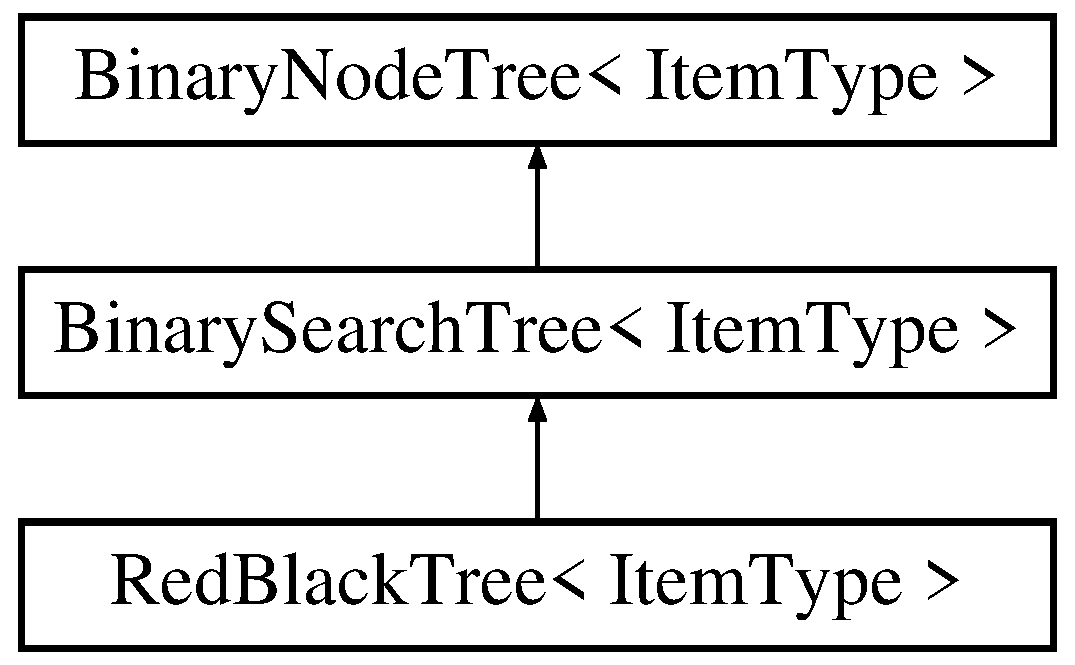
\includegraphics[height=2.000000cm]{class_binary_search_tree}
\end{center}
\end{figure}
\subsection*{Public Member Functions}
\begin{DoxyCompactItemize}
\item 
\hypertarget{class_binary_search_tree_acbe0ba28d119b4a36773d5d608938081}{}\label{class_binary_search_tree_acbe0ba28d119b4a36773d5d608938081} 
bool {\bfseries is\+Empty} () const
\item 
\hypertarget{class_binary_search_tree_a04eaf25b5dd9edabcbca44e323aac600}{}\label{class_binary_search_tree_a04eaf25b5dd9edabcbca44e323aac600} 
int {\bfseries get\+Height} () const
\item 
\hypertarget{class_binary_search_tree_a128756fb6e116279cf2c2b99afa02dfd}{}\label{class_binary_search_tree_a128756fb6e116279cf2c2b99afa02dfd} 
int {\bfseries get\+Number\+Of\+Nodes} () const
\item 
\hypertarget{class_binary_search_tree_ae07638c930af66e75601d9570a2ea2de}{}\label{class_binary_search_tree_ae07638c930af66e75601d9570a2ea2de} 
Item\+Type {\bfseries get\+Root\+Data} () const
\item 
\hypertarget{class_binary_search_tree_a7bb2a0da26e2e846981e2dc7a6ac101b}{}\label{class_binary_search_tree_a7bb2a0da26e2e846981e2dc7a6ac101b} 
void {\bfseries set\+Root\+Data} (Item\+Type \&new\+Entry)
\item 
\hypertarget{class_binary_search_tree_a56fc2830f911fe6e082df6ac8f4f6cce}{}\label{class_binary_search_tree_a56fc2830f911fe6e082df6ac8f4f6cce} 
bool {\bfseries add} (const Item\+Type \&new\+Data)
\item 
\hypertarget{class_binary_search_tree_ae3242f442fbd2ee75c1a026a7e023f86}{}\label{class_binary_search_tree_ae3242f442fbd2ee75c1a026a7e023f86} 
bool {\bfseries remove} (const Item\+Type \&target)
\item 
\hypertarget{class_binary_search_tree_ae691f40ac35ced8ef7d0661f4dcbdc8a}{}\label{class_binary_search_tree_ae691f40ac35ced8ef7d0661f4dcbdc8a} 
void {\bfseries clear} ()
\item 
\hypertarget{class_binary_search_tree_a3fee4b81cd95e3be7a6f9b0648b5b6de}{}\label{class_binary_search_tree_a3fee4b81cd95e3be7a6f9b0648b5b6de} 
Item\+Type {\bfseries get\+Entry} (const Item\+Type \&an\+Entry) const
\item 
\hypertarget{class_binary_search_tree_a744f02938ba3fe5006724188978fa56f}{}\label{class_binary_search_tree_a744f02938ba3fe5006724188978fa56f} 
void {\bfseries preorder\+Trav} (void visit(Item\+Type \&)) const
\item 
\hypertarget{class_binary_search_tree_a39b1fed377231ba7a118b60cb1c2238f}{}\label{class_binary_search_tree_a39b1fed377231ba7a118b60cb1c2238f} 
void {\bfseries inorder\+Trav} (void visit(Item\+Type \&)) const
\item 
\hypertarget{class_binary_search_tree_a1bd5beb35a142b659eebb445c289d347}{}\label{class_binary_search_tree_a1bd5beb35a142b659eebb445c289d347} 
void {\bfseries postorder\+Trav} (void visit(Item\+Type \&)) const
\end{DoxyCompactItemize}
\subsection*{Protected Member Functions}
\begin{DoxyCompactItemize}
\item 
\hypertarget{class_binary_search_tree_abd1859220c1ba567bb1ff566e1eeacd9}{}\label{class_binary_search_tree_abd1859220c1ba567bb1ff566e1eeacd9} 
\hyperlink{class_binary_node}{Binary\+Node}$<$ Item\+Type $>$ $\ast$ {\bfseries place\+Node} (\hyperlink{class_binary_node}{Binary\+Node}$<$ Item\+Type $>$ $\ast$sub\+Tree\+Ptr, \hyperlink{class_binary_node}{Binary\+Node}$<$ Item\+Type $>$ $\ast$new\+Node\+Ptr)
\item 
\hypertarget{class_binary_search_tree_a60a411ec64c72701c33325e78d55ba11}{}\label{class_binary_search_tree_a60a411ec64c72701c33325e78d55ba11} 
\hyperlink{class_binary_node}{Binary\+Node}$<$ Item\+Type $>$ $\ast$ {\bfseries remove\+Value} (\hyperlink{class_binary_node}{Binary\+Node}$<$ Item\+Type $>$ $\ast$sub\+Tree\+Ptr, const Item\+Type \&target, bool \&is\+Successful)
\item 
\hypertarget{class_binary_search_tree_a3a78640dd0d8e2658eeba619ef5d9851}{}\label{class_binary_search_tree_a3a78640dd0d8e2658eeba619ef5d9851} 
\hyperlink{class_binary_node}{Binary\+Node}$<$ Item\+Type $>$ $\ast$ {\bfseries remove\+Node} (\hyperlink{class_binary_node}{Binary\+Node}$<$ Item\+Type $>$ $\ast$node\+To\+Remove\+Ptr)
\item 
\hypertarget{class_binary_search_tree_a0cc4ccebb32f56016905e9eb76d21f27}{}\label{class_binary_search_tree_a0cc4ccebb32f56016905e9eb76d21f27} 
\hyperlink{class_binary_node}{Binary\+Node}$<$ Item\+Type $>$ $\ast$ {\bfseries remove\+Leftmost\+Node} (\hyperlink{class_binary_node}{Binary\+Node}$<$ Item\+Type $>$ $\ast$node\+Ptr, Item\+Type \&inorder\+Successor)
\item 
\hypertarget{class_binary_search_tree_a91096bb57439c2551bc65de4f441b13d}{}\label{class_binary_search_tree_a91096bb57439c2551bc65de4f441b13d} 
\hyperlink{class_binary_node}{Binary\+Node}$<$ Item\+Type $>$ $\ast$ {\bfseries find\+Node} (\hyperlink{class_binary_node}{Binary\+Node}$<$ Item\+Type $>$ $\ast$tree\+Ptr, const Item\+Type \&target) const
\item 
\hypertarget{class_binary_search_tree_ad98b67dc1e47557e51cc5553ab3f2d25}{}\label{class_binary_search_tree_ad98b67dc1e47557e51cc5553ab3f2d25} 
void {\bfseries clear\+Tree} (\hyperlink{class_binary_node}{Binary\+Node}$<$ Item\+Type $>$ $\ast$sub\+Tree\+Ptr)
\end{DoxyCompactItemize}


The documentation for this class was generated from the following files\+:\begin{DoxyCompactItemize}
\item 
\hyperlink{_binary_search_tree_8h}{Binary\+Search\+Tree.\+h}\item 
\hyperlink{_binary_search_tree_8cpp}{Binary\+Search\+Tree.\+cpp}\end{DoxyCompactItemize}

\hypertarget{class_red_black_tree}{}\section{Red\+Black\+Tree$<$ Item\+Type $>$ Class Template Reference}
\label{class_red_black_tree}\index{Red\+Black\+Tree$<$ Item\+Type $>$@{Red\+Black\+Tree$<$ Item\+Type $>$}}
Inheritance diagram for Red\+Black\+Tree$<$ Item\+Type $>$\+:\begin{figure}[H]
\begin{center}
\leavevmode
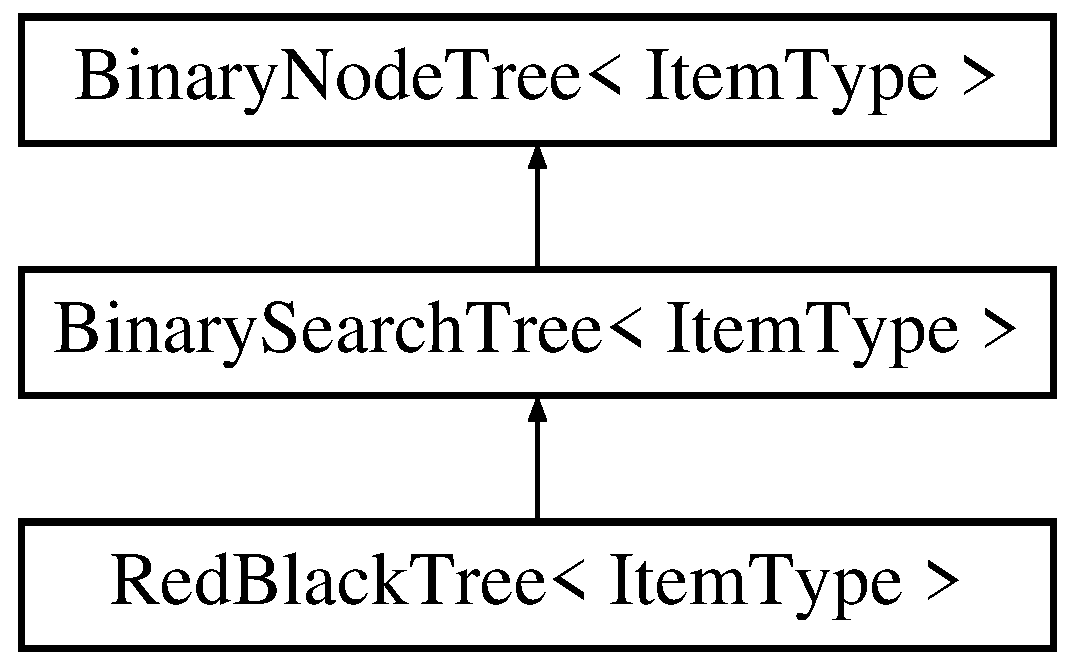
\includegraphics[height=3.000000cm]{class_red_black_tree}
\end{center}
\end{figure}
\subsection*{Public Member Functions}
\begin{DoxyCompactItemize}
\item 
\hypertarget{class_red_black_tree_af3713cafd8989d89f3685f56c7f36702}{}\label{class_red_black_tree_af3713cafd8989d89f3685f56c7f36702} 
bool {\bfseries is\+Empty} () const
\item 
\hypertarget{class_red_black_tree_ac8c0d6f98d9c7cc53b15d9364014fbcc}{}\label{class_red_black_tree_ac8c0d6f98d9c7cc53b15d9364014fbcc} 
int {\bfseries get\+Height} () const
\item 
\hypertarget{class_red_black_tree_ac08bdca9a79721e58b7a57a7a3921ba6}{}\label{class_red_black_tree_ac08bdca9a79721e58b7a57a7a3921ba6} 
int {\bfseries get\+Number\+Of\+Nodes} () const
\item 
\hypertarget{class_red_black_tree_a6b7d3b3463133035a5864bc8c25bf0fc}{}\label{class_red_black_tree_a6b7d3b3463133035a5864bc8c25bf0fc} 
Item\+Type {\bfseries get\+Root\+Data} () const
\item 
\hypertarget{class_red_black_tree_ace37f9b72094ce968461f54f4374b9ce}{}\label{class_red_black_tree_ace37f9b72094ce968461f54f4374b9ce} 
void {\bfseries set\+Root\+Data} (Item\+Type \&new\+Entry)
\item 
\hypertarget{class_red_black_tree_aa2b3d785de13923e62f42a5f99d913d7}{}\label{class_red_black_tree_aa2b3d785de13923e62f42a5f99d913d7} 
bool {\bfseries add} (const Item\+Type \&new\+Data)
\item 
\hypertarget{class_red_black_tree_a9c196b5513df89b2daabad5c59917268}{}\label{class_red_black_tree_a9c196b5513df89b2daabad5c59917268} 
bool {\bfseries remove} (const Item\+Type \&target)
\item 
\hypertarget{class_red_black_tree_a3c359138ca12b255645857a7eeb68ff4}{}\label{class_red_black_tree_a3c359138ca12b255645857a7eeb68ff4} 
void {\bfseries clear} ()
\item 
\hypertarget{class_red_black_tree_aa966683700681d154286668bb38871c4}{}\label{class_red_black_tree_aa966683700681d154286668bb38871c4} 
Item\+Type {\bfseries get\+Entry} (const Item\+Type \&an\+Entry) const
\item 
\hypertarget{class_red_black_tree_a3eb7fc10aade40772a734f9fd3168a71}{}\label{class_red_black_tree_a3eb7fc10aade40772a734f9fd3168a71} 
void {\bfseries preorder\+Trav} (void visit(Item\+Type \&)) const
\item 
\hypertarget{class_red_black_tree_a0675414d0278dcb0a4f4e27fd5e8dcd4}{}\label{class_red_black_tree_a0675414d0278dcb0a4f4e27fd5e8dcd4} 
void {\bfseries inorder\+Trav} (Item\+Type \&) const
\item 
\hypertarget{class_red_black_tree_a420f5aee2e3f306985ce6bd80b7f8d70}{}\label{class_red_black_tree_a420f5aee2e3f306985ce6bd80b7f8d70} 
void {\bfseries postorder\+Trav} (void visit(Item\+Type \&)) const
\end{DoxyCompactItemize}
\subsection*{Additional Inherited Members}


The documentation for this class was generated from the following files\+:\begin{DoxyCompactItemize}
\item 
\hyperlink{_red_black_tree_8h}{Red\+Black\+Tree.\+h}\item 
\hyperlink{_red_black_tree_8cpp}{Red\+Black\+Tree.\+cpp}\end{DoxyCompactItemize}

\chapter{File Documentation}
\hypertarget{_binary_node_8cpp}{}\section{Binary\+Node.\+cpp File Reference}
\label{_binary_node_8cpp}\index{Binary\+Node.\+cpp@{Binary\+Node.\+cpp}}


Implementation file for the Binary Node class.  




\subsection{Detailed Description}
Implementation file for the Binary Node class. 

\begin{DoxyAuthor}{Author}
Willis Allstead
\end{DoxyAuthor}
\begin{DoxyVersion}{Version}
0.\+5 
\end{DoxyVersion}

\hypertarget{_binary_node_8h}{}\section{Binary\+Node.\+h File Reference}
\label{_binary_node_8h}\index{Binary\+Node.\+h@{Binary\+Node.\+h}}


Header file for the Binary Node class.  


{\ttfamily \#include \char`\"{}Binary\+Node.\+cpp\char`\"{}}\newline
\subsection*{Classes}
\begin{DoxyCompactItemize}
\item 
class \hyperlink{class_binary_node}{Binary\+Node$<$ Item\+Type $>$}
\end{DoxyCompactItemize}


\subsection{Detailed Description}
Header file for the Binary Node class. 

\begin{DoxyAuthor}{Author}
Willis Allstead
\end{DoxyAuthor}
Specifies the members of the \hyperlink{class_binary_node}{Binary\+Node} class

\begin{DoxyVersion}{Version}
0.\+5 
\end{DoxyVersion}

\hypertarget{_binary_node_tree_8cpp}{}\section{Binary\+Node\+Tree.\+cpp File Reference}
\label{_binary_node_tree_8cpp}\index{Binary\+Node\+Tree.\+cpp@{Binary\+Node\+Tree.\+cpp}}


Implementation file for the Binary Node Tree class.  




\subsection{Detailed Description}
Implementation file for the Binary Node Tree class. 

\begin{DoxyAuthor}{Author}
Willis Allstead
\end{DoxyAuthor}
\begin{DoxyVersion}{Version}
0.\+5 
\end{DoxyVersion}

\hypertarget{_binary_node_tree_8h}{}\section{Binary\+Node\+Tree.\+h File Reference}
\label{_binary_node_tree_8h}\index{Binary\+Node\+Tree.\+h@{Binary\+Node\+Tree.\+h}}


Header file for the Binary Node Tree class.  


{\ttfamily \#include $<$algorithm$>$}\newline
{\ttfamily \#include \char`\"{}Binary\+Node.\+h\char`\"{}}\newline
{\ttfamily \#include \char`\"{}Binary\+Node\+Tree.\+cpp\char`\"{}}\newline
\subsection*{Classes}
\begin{DoxyCompactItemize}
\item 
class \hyperlink{class_binary_node_tree}{Binary\+Node\+Tree$<$ Item\+Type $>$}
\end{DoxyCompactItemize}


\subsection{Detailed Description}
Header file for the Binary Node Tree class. 

\begin{DoxyAuthor}{Author}
Willis Allstead
\end{DoxyAuthor}
Specifies the members of the Binary Node Tree class

\begin{DoxyVersion}{Version}
0.\+5 
\end{DoxyVersion}

\hypertarget{_binary_search_tree_8cpp}{}\section{Binary\+Search\+Tree.\+cpp File Reference}
\label{_binary_search_tree_8cpp}\index{Binary\+Search\+Tree.\+cpp@{Binary\+Search\+Tree.\+cpp}}


Implementation file for the Binary Search Tree class.  




\subsection{Detailed Description}
Implementation file for the Binary Search Tree class. 

\begin{DoxyAuthor}{Author}
Willis Allstead
\end{DoxyAuthor}
\begin{DoxyVersion}{Version}
0.\+5 
\end{DoxyVersion}

\hypertarget{_binary_search_tree_8h}{}\section{Binary\+Search\+Tree.\+h File Reference}
\label{_binary_search_tree_8h}\index{Binary\+Search\+Tree.\+h@{Binary\+Search\+Tree.\+h}}


Header file for the Binary Search Tree class.  


{\ttfamily \#include \char`\"{}Binary\+Node.\+h\char`\"{}}\newline
{\ttfamily \#include \char`\"{}Binary\+Node\+Tree.\+h\char`\"{}}\newline
{\ttfamily \#include \char`\"{}Binary\+Search\+Tree.\+cpp\char`\"{}}\newline
\subsection*{Classes}
\begin{DoxyCompactItemize}
\item 
class \hyperlink{class_binary_search_tree}{Binary\+Search\+Tree$<$ Item\+Type $>$}
\end{DoxyCompactItemize}


\subsection{Detailed Description}
Header file for the Binary Search Tree class. 

\begin{DoxyAuthor}{Author}
Willis Allstead
\end{DoxyAuthor}
Specifies the members of the Binary Search Tree class

\begin{DoxyVersion}{Version}
0.\+5 
\end{DoxyVersion}

\hypertarget{_p_a07_8cpp}{}\section{P\+A07.\+cpp File Reference}
\label{_p_a07_8cpp}\index{P\+A07.\+cpp@{P\+A07.\+cpp}}


Main driver for project 7.  


{\ttfamily \#include $<$iostream$>$}\newline
{\ttfamily \#include \char`\"{}Red\+Black\+Tree.\+h\char`\"{}}\newline
\subsection*{Functions}
\begin{DoxyCompactItemize}
\item 
\hypertarget{_p_a07_8cpp_a226f05ce9b96692a51f80edc81c9d71d}{}\label{_p_a07_8cpp_a226f05ce9b96692a51f80edc81c9d71d} 
bool {\bfseries exists\+In\+Array} (int to\+Check, int arr\mbox{[}$\,$\mbox{]}, int count)
\item 
\hypertarget{_p_a07_8cpp_ae66f6b31b5ad750f1fe042a706a4e3d4}{}\label{_p_a07_8cpp_ae66f6b31b5ad750f1fe042a706a4e3d4} 
int {\bfseries main} ()
\end{DoxyCompactItemize}
\subsection*{Variables}
\begin{DoxyCompactItemize}
\item 
\hypertarget{_p_a07_8cpp_aea314b8817a5900f77886bd8f5c73ccd}{}\label{_p_a07_8cpp_aea314b8817a5900f77886bd8f5c73ccd} 
const int {\bfseries num\+Values} = 1000
\end{DoxyCompactItemize}


\subsection{Detailed Description}
Main driver for project 7. 

\begin{DoxyAuthor}{Author}
Willis Allstead
\end{DoxyAuthor}
\begin{DoxyVersion}{Version}
1.\+0 
\end{DoxyVersion}

\hypertarget{_red_black_tree_8cpp}{}\section{Red\+Black\+Tree.\+cpp File Reference}
\label{_red_black_tree_8cpp}\index{Red\+Black\+Tree.\+cpp@{Red\+Black\+Tree.\+cpp}}


Implementation file for the Red Black Tree class.  




\subsection{Detailed Description}
Implementation file for the Red Black Tree class. 

\begin{DoxyAuthor}{Author}
Willis Allstead
\end{DoxyAuthor}
\begin{DoxyVersion}{Version}
0.\+5 
\end{DoxyVersion}

\hypertarget{_red_black_tree_8h}{}\section{Red\+Black\+Tree.\+h File Reference}
\label{_red_black_tree_8h}\index{Red\+Black\+Tree.\+h@{Red\+Black\+Tree.\+h}}


Header file for the Red Black Tree class.  


{\ttfamily \#include \char`\"{}Binary\+Node.\+h\char`\"{}}\newline
{\ttfamily \#include \char`\"{}Binary\+Search\+Tree.\+h\char`\"{}}\newline
{\ttfamily \#include \char`\"{}Red\+Black\+Tree.\+cpp\char`\"{}}\newline
\subsection*{Classes}
\begin{DoxyCompactItemize}
\item 
class \hyperlink{class_red_black_tree}{Red\+Black\+Tree$<$ Item\+Type $>$}
\end{DoxyCompactItemize}


\subsection{Detailed Description}
Header file for the Red Black Tree class. 

\begin{DoxyAuthor}{Author}
Willis Allstead
\end{DoxyAuthor}
Specifies the members of the Red Black Tree class

\begin{DoxyVersion}{Version}
0.\+5 
\end{DoxyVersion}

%--- End generated contents ---

% Index
\backmatter
\newpage
\phantomsection
\clearemptydoublepage
\addcontentsline{toc}{chapter}{Index}
\printindex

\end{document}
